\documentclass[12pt]{article}

\title{ET4340 Electronics for Quantum Computing\\Homework 2}
\author{
    Mick van Gelderen\\4091566
}
\date{November 2013}

\usepackage[utf8]{inputenc}
\usepackage[a4paper,margin=2.2cm]{geometry}
\usepackage{natbib}
\usepackage{graphicx}
\usepackage{listings}
\usepackage{framed}
\usepackage{mathtools}
\usepackage{braket}
\usepackage{ifmtarg}
\usepackage{multirow}

\newcommand{\pauli}[1]{
    \ensuremath{
        \begin{pmatrix}
            \if#1x
                0 & 1 \\
                1 & 0 \\
            \fi\if#1y
                0 & -i \\
                i & 0 \\
            \fi\if#1z
                1 & 0 \\
                0 & -1 \\
            \fi
        \end{pmatrix}
    }
}

\setlength{\parindent}{0cm}

\newcommand{\paulisigma}[1]{%
    \ensuremath{\sigma{}_{#1}}%
}

\newcommand{\pmat}[1]{\begin{pmatrix}#1\end{pmatrix}}
\newcommand{\rsqrt}[1]{\ensuremath{\frac{1}{\sqrt{#1}}}}

\setlength{\parskip}{0.5em plus4mm minus3mm}
\newenvironment{answer}{\begingroup\setlength{\leftskip}{-\leftmargin}\begin{framed}}{\end{framed}\endgroup}

\newcommand{\CNOT}[1]{\ensuremath{\texttt{CNOT}_{#1}}}
\newcommand{\CPHASE}[1]{\ensuremath{\texttt{CPHASE}_{#1}}}
\newcommand{\SWAP}[1]{\ensuremath{\texttt{SWAP}_{#1}}}

\begin{document}

\maketitle
\hfill\\\\\\

\paragraph{Problem 1: The Bell basis} \hfill \\

In class, we introduced the \emph{Bell states}
\begin{align*}
    \ket{\Psi_+} &= \rsqrt{2} (\ket{01} + \ket{10}) \\
    \ket{\Psi_-} &= \rsqrt{2} (\ket{01} - \ket{10}) \\
    \ket{\Phi_+} &= \rsqrt{2} (\ket{00} + \ket{11}) \\
    \ket{\Phi_-} &= \rsqrt{2} (\ket{00} - \ket{11}) \\
\end{align*}

Like the computational basis ${\ket{00}, \ket{01}, \ket{10}, \ket{11}}$, this set of states forms a basis for the fourdimensional Hilbert space of two qubits. Show that this basis is ortho-normal. That is:

\begin{enumerate}

    \item Show that the inner product of every Bell state with itself is unity. In other words, show that $\braket{\Upsilon|\Upsilon} = 1 | \forall \Upsilon \in \{\Psi_+, \Psi_-, \Phi_+, \Phi_-\}$.

    \begin{answer}
        The bell states can be written as simple vectors as follows:
        \begin{align*}{2}
            \ket{\Psi_+} &= \rsqrt{2} \pmat{0 & 1 & \phantom{-}1 & \phantom{-}0}^\top \\
            \ket{\Psi_-} &= \rsqrt{2} \pmat{0 & 1 &           -1 & \phantom{-}0}^\top \\
            \ket{\Phi_+} &= \rsqrt{2} \pmat{1 & 0 & \phantom{-}0 & \phantom{-}1}^\top \\
            \ket{\Phi_-} &= \rsqrt{2} \pmat{1 & 0 & \phantom{-}0 &           -1}^\top \\
        \end{align*}
        It is very easy to see that for each vector, taking the inner product with itself results in 1. For example:
        \begin{align*}
            \braket{\Psi_+|\Psi_+} = \left(\rsqrt{2}\right)^2 \cdot (0^2 + 1^2 + 1^2 + 0^2) = 1
        \end{align*}
    \end{answer}

    \item Show that the inner product of every Bell state with every other bell state equals zero.

    \begin{answer}
        Since the inner product is commutative we only have to do a small set of computations. Also, it is easy to see that the inner product between a $\Psi$ and a $\Phi$ Bell state equals $0$ since there is a zero in every row. So the remaining cases are:
        \begin{alignat*}{8}
            \braket{\Psi_+|\Psi_-} &= \left(\rsqrt{2}\right)^2 \cdot (0^2 && + && 1^2 && + && 1\cdot(-1) && + && 0^2    && ) = 0 \\
            \braket{\Phi_+|\Phi_-} &= \left(\rsqrt{2}\right)^2 \cdot (1^2 && + && 0^2 && + && 0^2    && + && 1\cdot(-1) && ) = 0 \\
        \end{alignat*}
    \end{answer}

    \item Write a matrix that transforms the coordinates of a state in the computational basis to the coordinates of the same state in the Bell basis. To be clear, find a matrix $M$ that translates $\ket{00}$ to $\ket{\Psi_+}$, $\ket{01}$ to $\ket{\Psi_-}$, and so forth.

    \begin{answer}
        Lets say we want to express the state $\ket{00} = \pmat{1 & 0 & 0 & 0}$ in the computational basis in the Bell basis. We must find a lineair combination of the bell states that adds up to $\ket{00}$.

        We could do this by reducing a matrix but that should not be necessary. You can see that we need to add $\ket{\Phi_+}$ and $\ket{\Phi_-}$ and normalize it.

        \begin{alignat*}{2}
              \ket{00}
                &= x \cdot \left(\ket{\Phi_+} + \ket{\Phi_-}\right) && \\
                &= x \cdot 2 \cdot \rsqrt{2}\ket{00} && \text{ where } x \cdot 2 \cdot \rsqrt{2} = 1 \text{ so } x = \rsqrt{2} \\
                &= \rsqrt{2} \cdot \left(\ket{\Phi_+} + \ket{\Phi_-}\right) \\
                &= \rsqrt{2} \cdot \pmat{0 & 0 & 1 & 1}^\top \\
        \end{alignat*}

        If we repeat these steps for all the computational states we get the following matrix:

        \begin{align*}
            M = \rsqrt{2} \cdot \pmat{
                0 & 1 & \phantom{-}1 & \phantom{-}0 \\
                0 & 1 &           -1 & \phantom{-}0 \\
                1 & 0 & \phantom{-}0 & \phantom{-}1 \\
                1 & 0 & \phantom{-}0 &           -1 \\
            }
        \end{align*}
    \end{answer}

\end{enumerate}

\paragraph{Problem 2: Generalized \CPHASE{} gates} \hfill \\

\begin{enumerate}
    \item Write the four-by-four matrix transformation which flips the phase of the green qubit and does nothing to the red qubit, i.e., implements $Z \otimes I$.

    \begin{answer}
        Lets notate the two-qubit state as $\ket{gr}$. It can be proven that $\left(A \cdot \ket{g}\right) \otimes \left(B \cdot \ket{r}\right) = \left(A \otimes B\right) \cdot \left(\ket{g} \otimes \ket{r}\right)$. This property can be used to conjure multi-cubit transformations from single-cubit transformations.

        To find the transformation that flips the green and retains the red we compute $Z \otimes I$

        \begin{align*}
            Z \otimes I
                &= \left(\begin{array}{c|c}
                    Z_{1,1}I & Z_{1,2}I \\\hline
                    Z_{2,1}I & Z_{2,2}I
                \end{array}\right) \\
                &= \pmat{1&&&\\&1&&\\&&-1&\\&&&-1}
        \end{align*}
    \end{answer}

    \item Now do the reverse, flip the red qubit and do nothing to the green qubit.

    \begin{answer}
        \begin{align*}
            I \otimes Z = \pmat{1&&&\\&-1&&\\&&1&\\&&&-1}
        \end{align*}
    \end{answer}

    \item Give the matrix which flips the phase of the green qubit if and only if the red qubit is in $\ket{0}$.

    \begin{answer}
        This gate is a lot like the $Z \otimes I$ transformation except that we don't want to flip when the red qubit is in $\ket{1}$. So we flip the sign of the fourth column which corresponds to $\ket{11}$:

        \begin{align*}
            \CPHASE{s}\footnotemark = \pmat{1&&&\\&1&&\\&&-1&\\&&&1}
        \end{align*}
    \end{answer}

    \footnotetext{$\CPHASE{s}$ denotes the gate discussed in class}

    Similarly, we can imagine two more generalized \CPHASE{} gates. Show by example how using Z gates we can change any one of these transformations into any of the other three.

    \begin{answer}
        You can calculate $(Z \otimes I)\CPHASE{s}$ and $(Z \otimes Z)\CPHASE{s}$ to get two new gates with a $-1$ in the respectively the fourth and second columns (since $Z \otimes Z$ has $\pmat{1&-1&-1&1}$ as the diagonal).
    \end{answer}

\end{enumerate}

\paragraph{Problem 3: From \CNOT{} to \CPHASE{} using experimentalist's one-qubit gates} \hfill \\

In class we discussed that \CPHASE{} = $H_g\CNOT{rg}H_g$.

\begin{enumerate}
    \item Show that $\CPHASE{} = R_{y,g}(-\frac{\pi}{2})\CNOT{rg}R_{y,g}(\frac{\pi}{2})$.

    \begin{answer}
        Lets start with computing $R_{y}(\pm\frac{\pi}{2})$:
        \begin{align*}
            R_y(-\frac{\pi}{2}) &= \cos(-\frac{\pi}{4})I - i\sin(-\frac{\pi}{4})Y \\
                &= \rsqrt{2}I + i\rsqrt{2}\pmat{0 & -i \\ i & 0} \\
                &= \rsqrt{2}\pmat{1 & -1 \\ 1 & 1} \\
            R_y(\frac{\pi}{2}) &= \cos(\frac{\pi}{4})I - i\sin(\frac{\pi}{4})Y \\
                &= \rsqrt{2}I - i\rsqrt{2}\pmat{0 & -i \\ i & 0} \\
                &= \rsqrt{2}\pmat{1 & 1 \\ -1 & 1}
        \end{align*}
        By using the lessons learnt in the previous assignment we can compute the transformation matrix for the operation $\left(R_{y}(-\frac{\pi}{2}) \otimes I\right)\CNOT{rg}\left(R_{y}(\frac{\pi}{2}) \otimes I\right)\ket{gr}$
        \begin{align*}
            M &= \frac{1}{2}
                \pmat{1 & 0 & -1 & 0 \\ 0 & 1 & 0 & -1 \\ 1 & 0 & 1 & 0 \\ 0 & 1 & 0 & 1}
                \pmat{1 & 0 & 0 & 0 \\ 0 & 0 & 0 & 1 \\ 0 & 0 & 1 & 0 \\ 0 & 1 & 0 & 0}
                \pmat{1 & 0 & 1 & 0 \\ 0 & 1 & 0 & 1 \\ -1 & 0 & 1 & 0 \\ 0 & -1 & 0 & 1} \\
            &= \frac{1}{2}
                \pmat{1 & 0 & -1 & 0 \\ 0 & 1 & 0 & -1 \\ 1 & 0 & 1 & 0 \\ 0 & 1 & 0 & 1}
                \pmat{1 & 0 & 1 & 0 \\ 0 & -1 & 0 & 1 \\ -1 & 0 & 1 & 0 \\ 0 & 1 & 0 & 1} \\
            &= \frac{1}{2}
                \pmat{2 & 0 & 0 & 0 \\ 0 & -2 & 0 & 0 \\ 0 & 0 & 2 & 0 \\ 0 & 0 & 0 & 2}
        \end{align*}
        So $M$ is actually a \CPHASE{} gate.
    \end{answer}

    \item Draw the quantum circuit implementing these three operations.

    \begin{answer}
        \centering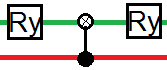
\includegraphics{bestpaintjob2013.png}
    \end{answer}
\end{enumerate}

\paragraph{Problem 4: The \SWAP{} operation} \hfill \\

The two-qubit unitary \SWAP{}, as the name implies, exchanges the quantum states of the green and red qubits, i.e., it implements the transformation $\ket{\psi} \otimes \ket{\phi} \rightarrow \ket{\phi} \otimes \ket{\psi}$. In quantum circuit language, the \SWAP{} gate is notated as a line between the qubits with crosses at the intersections.

\begin{enumerate}
    \item Write the four-by-four matrix representing this unitary transformation.

    \begin{answer}
        $\ket{00}$ and $\ket{11}$ are unaffected. $\ket{01}$ and $\ket{10}$ are interchanged thus the matrix will be:
        \begin{align*}
            \SWAP{} = \pmat{1 & 0 & 0 & 0 \\ 0 & 0 & 1 & 0 \\ 0 & 1 & 0 & 0 \\ 0 & 0 & 0 & 1}
        \end{align*}
    \end{answer}

    \item Show that $\SWAP{} = \CNOT{rg}\CNOT{gr}\CNOT{rg}$

    \begin{answer}
        This is a simple matrix multiplication and it turns out to be correct.
    \end{answer}

    \item Show that $\SWAP{} = \CNOT{gr}\CNOT{rg}\CNOT{gr}$

    \begin{answer}
        This is a simple matrix multiplication and it turns out to be correct.
    \end{answer}
\end{enumerate}

\paragraph{Problem 5: Measurements on Bell states} \hfill \\ \hfill \\

Edoardo and Chris each have one qubit from a pair prepared in the Bell state $\ket{\Phi_+}$.

\begin{enumerate}
    \item Edoardo and Chris agree to each perform a measurement of $Z$ on their qubit. Edoardo measures $-1$. Can he predict the result of Chris' measurement?

    \begin{answer}
        No, the qubits in the Bell states are entangled. Performing a measurement with respect to any angle on one of the qubits will change both of the qubits.
    \end{answer}

    \item Suppose that instead Edoardo and Chris agree to each perform a measurement of $X$ on their qubit. Edoardo measures $+1$. Can he predict the result of Chris' measurement?

    \begin{answer}
        Again, no.
    \end{answer}

    \item Lastly, suppose that they agree that Edoardo measure $Y$ on this qubit and that Chris measures $Z$ on his. Edoardo measures $-1$. Can he predict the result of Chris' measurement?

    \begin{answer}
        Nope.
    \end{answer}
\end{enumerate}

\paragraph{Problem 6: Gate by measurement} \hfill \\

Consider the quantum circuit below. The initial state of the system is a product state with green qubit in $\ket{\Psi_{in}} = \alpha\ket{0} + \beta\ket{1}$ and the red qubit in $\ket{\phi} = \rsqrt{2} (\ket{0} + e^{i\phi}\ket{1})$.

\centering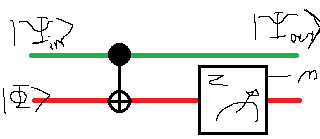
\includegraphics{problem6.png}

\begin{enumerate}
    \item Use the generalized Born rule to write the output state $\ket{\Psi_{out}}$ of the green qubit when the measurement result is $m = +1$. Show that for this case, the transformation $\ket{\Psi{in}} \rightarrow \ket{\Psi_{out}}$ is equivalent to a $z$ rotation of the green qubit by $\phi$.

    \begin{answer}
        Lets compute the circuit:
        \begin{align*}
            \CNOT{gr}(\pmat{\alpha \\ \beta} \otimes \rsqrt{2}\pmat{1 \\ e^{i\phi}}) = \pmat{ \alpha \\ \alpha{}e^{i\phi} \\ \beta{}e^{i\phi} \\ \beta }
        \end{align*}
        Since $m = +1$ when measuring the red qubit with respect to $Z$ we need to look at the states $\ket{00}$ and $\ket{10}$. So we get:
        \begin{align*}
            \ket{\Psi_{out}\Phi} &= \rsqrt{2}\left(\alpha\ket{00} + \beta{}e^{i\phi}\ket{10}\right) \\
                &= \rsqrt{2}\left(\alpha\ket{0} + \beta{}e^{i\phi}\ket{1}\right) \otimes \ket{0}
        \end{align*}
        We can see that only the green bit is affected and it was rotated by $\phi$.
    \end{answer}

    \item Similarly, write the output state of the green qubit when the measurement result is $m = -1$. For this case, what is the equivalent transformation $\ket{\Psi_{in}} \rightarrow \ket{\Psi_{out}}$?

    \begin{answer}
        Through similar means we get $\ket{\Psi_{out}} = \rsqrt{2}\left(\alpha{}e^{i\phi}\ket{0} + \beta\ket{1}\right)$. The transformation is an $y$ rotation of the green qubit by $\phi$.
    \end{answer}
\end{enumerate}
\end{document}

